\mode<article>

Las geometrías pueden definirse en archivos de texto plano con
extensión \texttt{.geo}. Estos archivos de geometría pueden
contener elementos de programación generales. Como se
esquematiza en la Figura \ref{FiguraEjemploGeometrias} 
es posible hacer comentarios y definir variables. La geometría
se genera mediante instrucciones con sintaxis específica. 

Debe tenerse en cuenta que la construcción de geometrías 
complejas es jerárquica. Por ejemplo, para definir un 
rectángulo deben definirse primero sus vértices, luego 
los lados, luego el borde (el lazo que contiene la superficie) y
por último su superficie. En las versiones más nuevas de gmsh
se han incluido instrucciones para definir estructuras complejas
en pocas instrucciones pero la estructura final de la 
matriz de conectividad refleja siempre estas estructuras jerárquicas. 
Las instrucciones siempre se terminan con un punto y coma (\texttt{;}).

\subsubsection{Factores de escala}
La definición de los puntos se realiza mediante la instrucción

\begin{figure}[h]
  \center
\begin{codeblock}
  \begin{BVerbatim}[fontfamily=courier]
Point( i ) = { x, y , z , fe } ;
\end{BVerbatim}
\end{codeblock}
\end{figure}

\noindent donde los tres primeros valores corresponden a las coordenadas
cartesianas del punto, y el cuarto valor corresponde al 
\emph{factor de escala}. Este número será de gran utilidad
en el momento de mallar los recintos de integración, i.e. al 
generar los elementos finitos que aproximan el recinto de interés. 
El valor del factor de escala corresponde con el tamaño 
característico de los elementos finitos alrededor del punto
definido. Por lo tanto, en un punto donde se necesita 
mayor resolución se puede usar un factor de escala pequeño,
mientras que en un punto donde no se requiere gran resolución
puede usarse un factor de escala grande. Los valores 
concretos dependen del tamaño característico en la geometría 
del problema en resolución. 

\begin{figure}
  \includeslide[width=\textwidth]{FrameEjemplosGeometrias}
  \caption{Generalidades del formato para escribir geometrías
  \label{FiguraEjemploGeometrias}
  }

\end{figure}

\mode*
\begin{frame}<presentation>[label=FrameEjemplosGeometrias]
  \frametitle{Geometrías}

  \begin{columns}

    \column{0.3\textwidth}
      \begin{codeblock}
	\scriptsize{
      \verbatiminput{./Ejemplos/chapa-clase.geo}
    }
    \end{codeblock}
    \column{0.7\textwidth}
    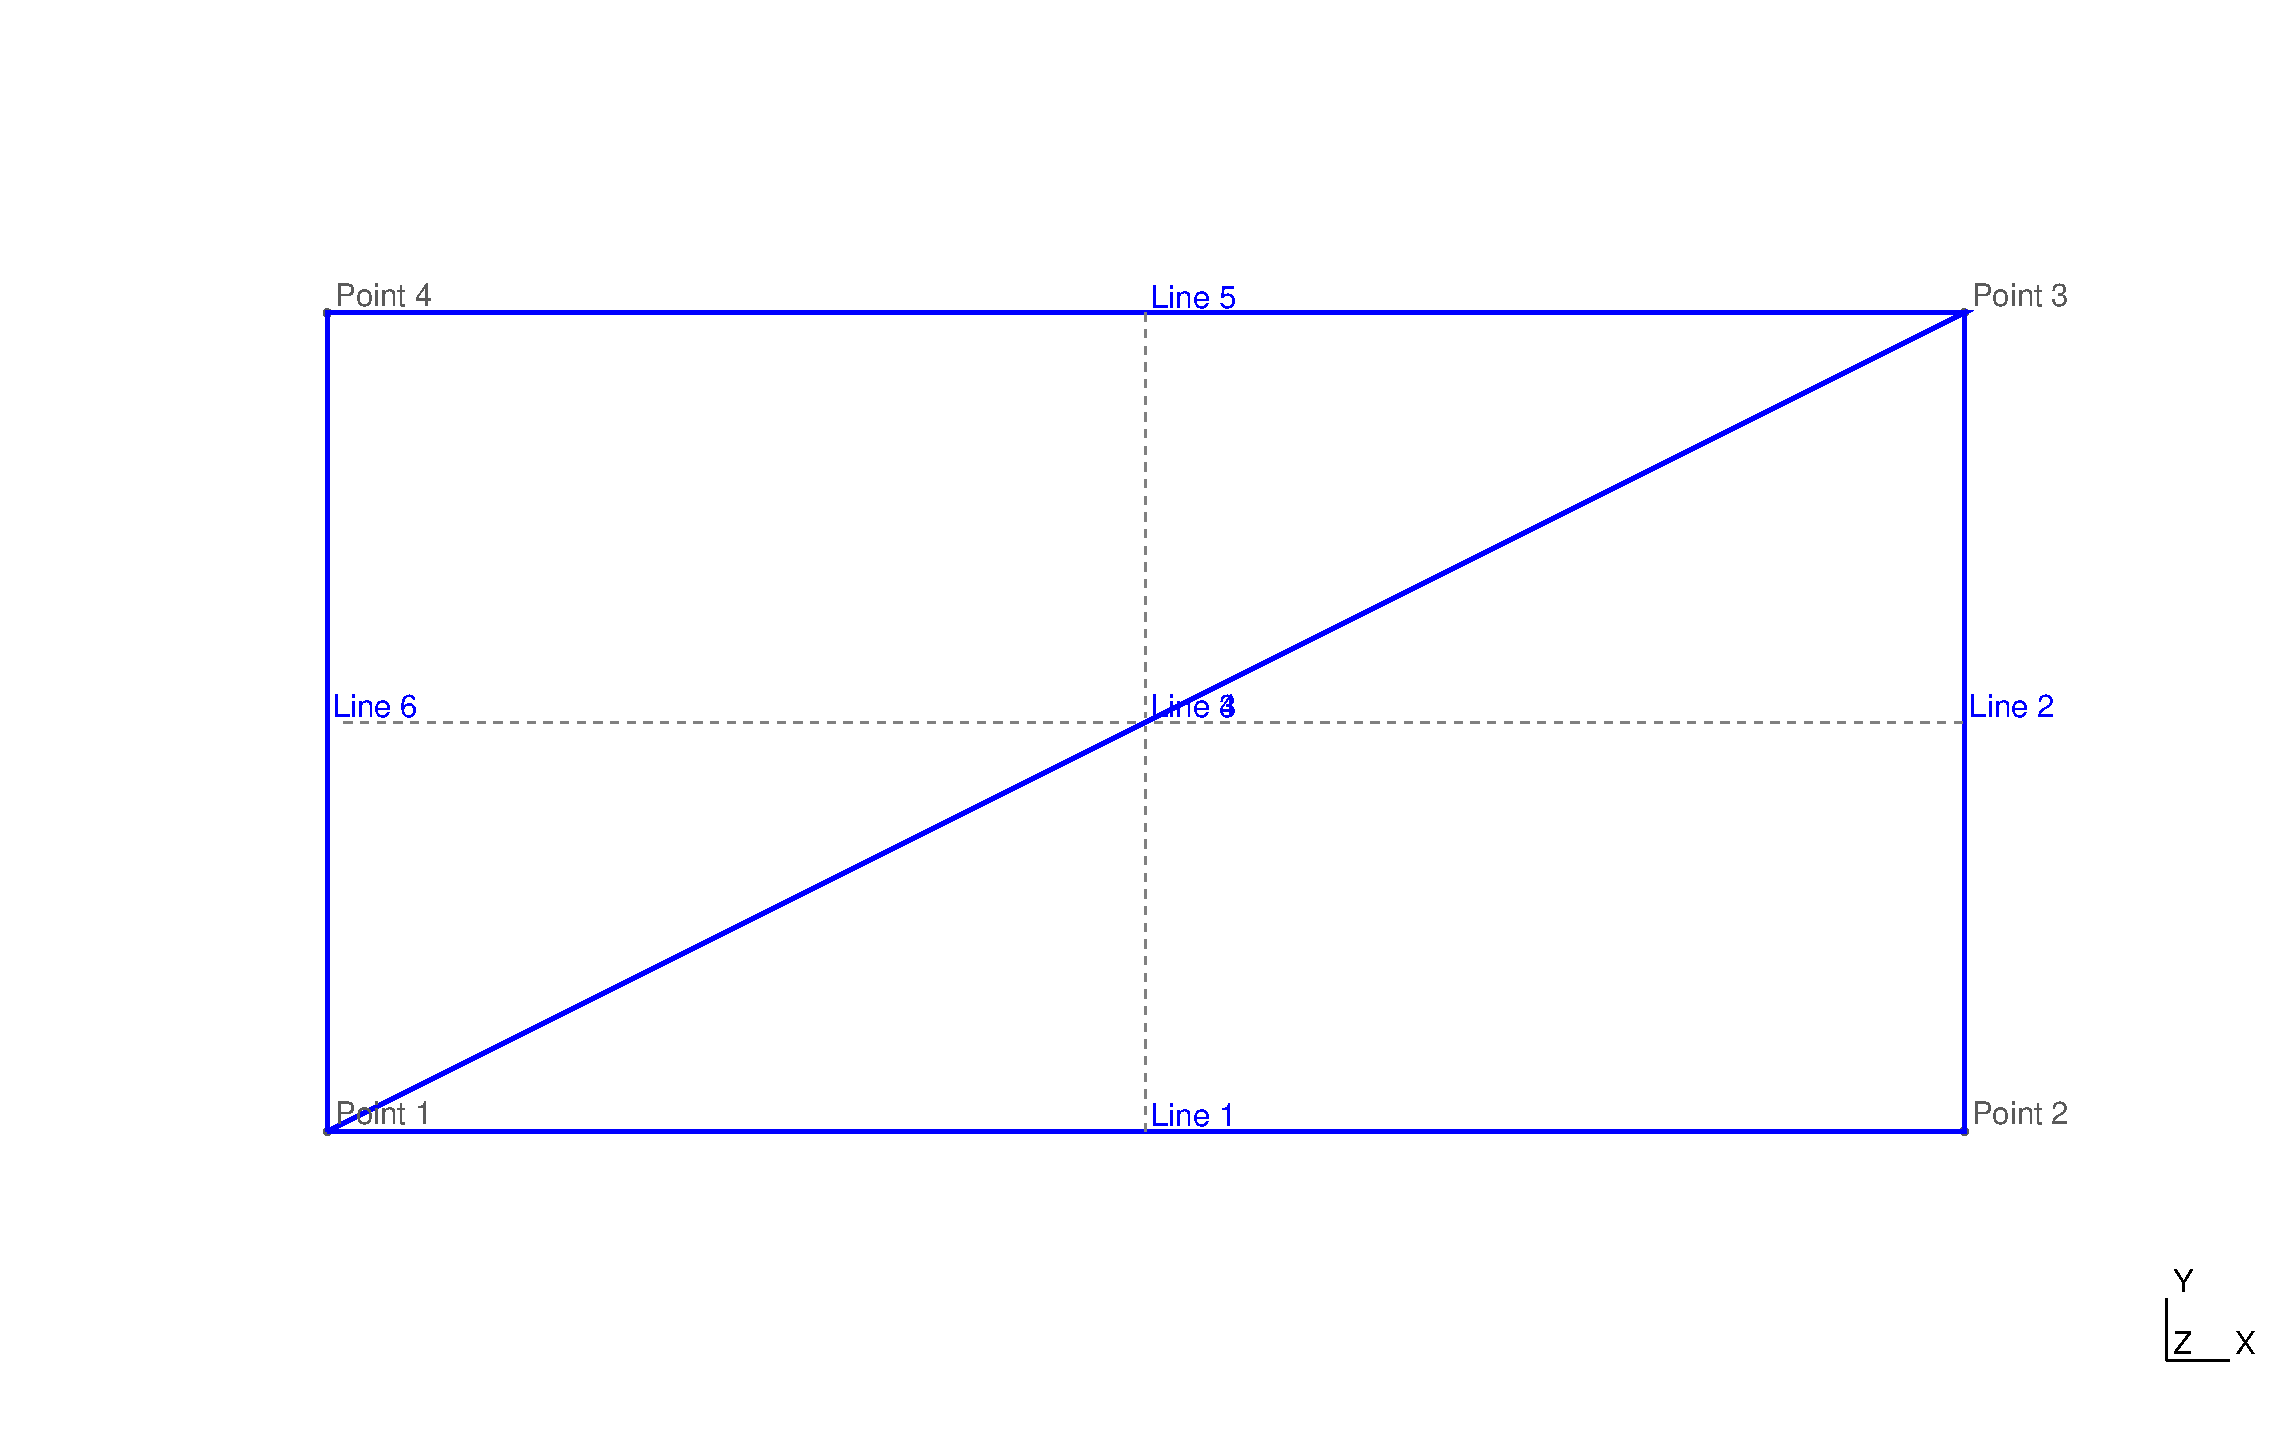
\includegraphics[width=\textwidth]{./Ejemplos/PuenteClase.pdf}
  \end{columns}


%  \includegraphics[width=\textwidth,page=6,bb=0cm 1cm 28cm 16cm,clip]{./Libreoffice/GMSH_fileformat.pdf}

\end{frame}

\mode<all>
